\documentclass[11pt,letterpaper]{article}

\usepackage{common}
\newboolean{solutionCopy}
\setboolean{solutionCopy}{false} % Toggle between solution copy and distro

\ifthenelse{\boolean{solutionCopy}}{
  \includeversion{solution}
}{
  \excludeversion{solution}
}
\newcommand{\class}{C}
\begin{document}

\ifthenelse{\boolean{solutionCopy}}{
\begin{center}
{\LARGE CS 181 Spring 2019 Section 9\\
Solution}
\end{center}
}{
  \begin{center}
{\LARGE CS 181 Spring 2019 Section 9}\\
\end{center}
}



%\pagebreak
%\newpage
%\thispagestyle{empty}
%\mbox{}
%\newpage
%\mbox{}

\section{Principal Component Analysis}

\subsection{Motivation}
In many supervised learning problems, we try to find rich features that increase the expressivity of our model. In practice, this often involves using basis functions to transform our input into a higher dimensional space (eg. given data $x$, using $x$ and $x^2$ as features, or using features learned by a neural network). 

However, sometimes we want to reduce the dimensionality of our data. There can be several reasons: fewer features are easier to interpret (we might want to know why our model outputs a certain diagnosis, and only some of the patient record details will be relevant); models with fewer features are easier to handle computationally; and our data might be arbitrarily high-dimensional because of noise, so we would like to access the lower-dimensional \emph{signal} from the data. One method for dimensionality reduction through \textbf{linear projections} of the original data is PCA. When reducing the dimensionality of our data from $m$ to $d$, PCA can be interpreted as minimizing the reconstruction loss of projecting data onto a $d$ basis vectors, or as maximizing the variance in data that can be explained by $d$ basis vectors. 

\subsection{Finding the lower dimensional representation}

To perform PCA, we first calculate the normalized \textbf{feature covariance} matrix after centering the data (by subtracting the mean image from each image):

  \[ \boldS = (\sum_{i=1}^n   \boldx_i\boldx_i^\top)  = \boldX^\top \boldX \]
  
We then decide how many dimensions $d$ out of the original $m$ that we want to keep in the final representation (for visualizations, often this will be $d=2$ or $d=3$). We then find the $d$ largest eigenvalues of $\boldS$. The $m \times 1$ eigenvectors ($\boldu_1, \dots ,\boldu_d$) corresponding to these eigenvalues will be our lower-dimensional basis. Thus, we reduce the dimensionality of a data point $\boldx$ by projecting it onto this basis - we combine the eigenvectors into the $d \times m$ matrix $\boldU$, and compute $\langle \boldx^\top\boldu_1, \boldx^\top\boldu_2, \ldots, \boldx^\top \boldu_d, \ldots, 0 \rangle = \boldU\boldx = \boldz$. $\boldz$ is called the reconstruction coefficients where $\boldU^\top \boldz$ is the reconstruction of $\boldx$.

\section{Bayesian Networks}

A Bayesian network is a graphical model that represents random variables and their dependencies using a directed acyclic graph. Bayesian networks are useful because they allow us to efficiently model joint distributions over many variables by taking advantage of the local dependencies between variables. With Bayesian networks, we can easily reason about conditional independence and perform inference on large joint distributions.

\subsection{D-separation rules}

Let $X_A$ and $X_B$ denote sets of variables that we are interested in reasoning about.
$X_A$ and $X_B$ are \textit{d-separated} by a set of evidence $X_E$ if \textbf{every} undirected path from $X_A$ to $X_B$ is ``blocked'' by $X_E$. A path is blocked by evidence $X_E$ if either:

\begin{enumerate}
\item There is a node $Z$ with non-converging arrows on the path, and $Z \in X_E$.

The shaded node indicates an evidence node.

\includegraphics[width=5cm]{block_nonconverge}

\item There is a node $Z$ with converging arrows on the path, and neither $Z$ nor its descendants are in $X_E$.

\includegraphics[width=4.5cm]{block_converging_3}
\end{enumerate}

Make sure to check \textbf{every} undirected path from $X_A$ to $X_B$. Within each path, only one node $Z$ needs to fall under one of the two cases described above for the whole path to be blocked.

If $X_A$ and $X_B$ are d-separated by $X_E$, then $X_A$ and $X_B$ are conditionally independent given $X_E$.
\newpage

\section{PCA}
\fbox{\parbox{\linewidth}{%
You are given the following data set:
\[ \boldx_1 = \begin{bmatrix} 1 \\ -1 \end{bmatrix}, \quad \boldx_2 = \begin{bmatrix} 1 \\ 2 \end{bmatrix}, \quad \boldx_3 = \begin{bmatrix} -2 \\ -1 \end{bmatrix} \]
You would like to use PCA to find a 1-dimensional representation of the data.
\begin{enumerate}
\item Plot the data set.
\item Compute the feature covariance matrix $\boldS$.
\item You find that $\boldS$ has eigenvector $[-1 \ 1]^\top$ with eigenvalue $3$ and eigenvector $[1 \ 1]^\top$ with eigenvalue $9$. What is the (normalized) basis vector $\boldu_1$ of your 1-dimensional representation? Add the basis vector $\boldu_1$ to your plot.
\item Compute the coefficients $z_1,z_2,z_3$. Add the lower-dimensional representations $z_1\boldu_1, z_2\boldu_1, z_3\boldu_1$ to your plot. Based on your plot, what is the relationship between $z_i\boldu_1$ and $\boldx_i$ with respect to the new basis?
\item Based on your plot, what would happen if you chose the unused eigenvector to be your basis vector?
\end{enumerate}
}}

\begin{solution}
\begin{enumerate}
\item \
\begin{center}
\begin{tikzpicture}[x=1cm,y=1cm]


\draw[latex-latex, thin, draw=gray] (-2,0)--(2,0) node [right] {}; % l'axe des abscisses
\draw[latex-latex, thin, draw=gray] (0,-2)--(0,2) node [above] {}; % l'axe des ordonnées

\foreach \Point in {(1,-1), (1,2), (-2,-1)}{
    \node at \Point {\textbullet};
}

% to ensure that the points are being properly centered:
\draw [dotted, gray] (-2,-2) grid (2,2);

\end{tikzpicture}
\end{center}

\item
\[ \boldS = \boldX^\top \boldX = \begin{bmatrix} 1 & -1 \\ 1 & 2 \\ -2 & -1 \end{bmatrix}^\top \begin{bmatrix} 1 & -1 \\ 1 & 2 \\ -2 & -1 \end{bmatrix} = \begin{bmatrix} 6 & 3 \\ 3 & 6 \end{bmatrix} \]
\item We select the eigenvectors with the largest eigenvalues for our basis, so our basis will contain a scalar multiple of $[1 \ 1]^\top$. Normalizing $[1 \ 1]^\top$ gives us that $\boldu_1 = [\frac{\sqrt{2}}{2} \ \frac{\sqrt{2}}{2}]^\top$.\\
\begin{center}
\begin{tikzpicture}[x=1cm,y=1cm]


\draw[latex-latex, thin, draw=gray] (-2,0)--(2,0) node [right] {};
\draw[latex-latex, thin, draw=gray] (0,-2)--(0,2) node [above] {};

\foreach \Point in {(1,-1), (1,2), (-2,-1)}{
    \node at \Point {\textbullet};
}

\draw [dotted, gray] (-2,-2) grid (2,2);

\draw[latex-latex, thin, draw=gray!30] (-2,-2)--(2,2) node {};
\draw[->] (0,0)--(0.7071,0.7071) node [above] {$\boldu_1$}; % basis vector

\end{tikzpicture}
\end{center}
\item 
\[ z_1 = \boldx_1^\top \boldu_1 = 0, \quad z_2 = \boldx_2^\top \boldu_1 = \frac{3\sqrt{2}}{2}, \quad z_3 = \boldx_3^\top \boldu_1 = -\frac{3\sqrt{2}}{2} \]
The open circles in the plot represent the lower-dimensional representation:
\begin{center}
\begin{tikzpicture}[x=1cm,y=1cm]


\draw[latex-latex, thin, draw=gray] (-2,0)--(2,0) node [right] {};
\draw[latex-latex, thin, draw=gray] (0,-2)--(0,2) node [above] {};

\foreach \Point in {(1,-1), (1,2), (-2,-1)}{
    \node at \Point {\textbullet};
}

\foreach \Point in {(0,0), (1.5,1.5), (-1.5,-1.5)}{
    \node at \Point {$\circ$};
}

\draw [dotted, gray] (-2,-2) grid (2,2);

\draw[latex-latex, thin, draw=gray!30] (-2,-2)--(2,2) node {};
\draw[->] (0,0)--(0.7071,0.7071) node [above] {$\boldu_1$}; % basis vector

\end{tikzpicture}
\end{center}
$z_i \boldu_1$ is the projection of $\boldx_i$ onto the basis vector.

\item If we chose $[-1 \ 1]^\top$ to be the basis of our new representation, then the representation would capture less of the variance in the data. For example, $\boldx_2$ and $\boldx_3$ would be represented by the same point.
\end{enumerate}
\end{solution}
\newpage
\section{Network Basics}

A patient goes to the doctor for a medical condition, and the doctor
suspects 3 diseases as the cause of the condition. The 3 diseases are
$D_1$, $D_2$, and $D_3$, and they are independent from each other
(given no other observations). There are 4 symptoms $S_1$, $S_2$,
$S_3$, and $S_4$, and the doctor wants to check for presence in order
to find the most probable cause.  $S_1$ can be caused by $D_1$, $S_2$
can be caused by $D_1$ and $D_2$, $S_3$ can be caused by $D_1$ and
$D_3$, and $S_4$ can be caused by $D_3$. Assume all random variables
are Bernoulli, i.e. the patient has the disease/symptom or not.
%
\begin{itemize}
\item \textbf{Q:} Draw a Bayesian network for this problem with the variable ordering  $D_1, D_2, D_3, S_1, S_2, S_3, S_4$. 

\begin{solution}
\textbf{A:} Note that there are many valid networks (depending on the chosen variable ordering), 
some more efficient (i.e. requiring fewer parameters) than others. Here is a 
compact representation that comes from variable ordering $D_1, D_2, D_3, S_1, S_2, S_3, S_4$. (Recall that 
all dependencies to earlier variables need to be indicated with edges).
%
\begin{figure}[htp]
% \begin{center}
%  \includegraphics[width=2.7in]{picture1.png}\\
%  \end{center}
\begin{center}
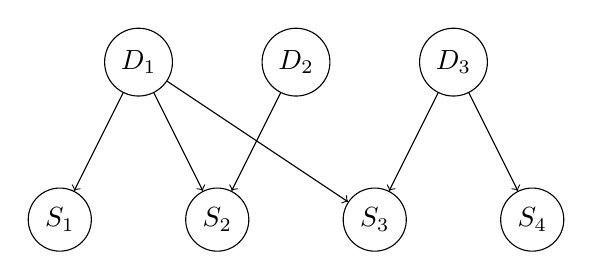
\begin{tikzpicture}
\begin{scope}[every node/.style={circle,draw}]
\node (D1) at (-2,1) {$D_1$};
\node (D2) at (0,1) {$D_2$};
\node (D3) at (2,1) {$D_3$};
\node (S1) at (-3,-1) {$S_1$};
\node (S2) at (-1,-1) {$S_2$};
\node (S3) at (1,-1) {$S_3$};
\node (S4) at (3,-1) {$S_4$};
\end{scope}

\begin{scope}[every edge/.style={draw}]
    \path [->] (D1) edge (S1);
    \path [->] (D1) edge (S2);
    \path [->] (D1) edge (S3);
    \path [->] (D2) edge (S2);
    \path [->] (D3) edge (S3);
    \path [->] (D3) edge (S4);
\end{scope}
\end{tikzpicture}
\end{center}
\end{figure}

\end{solution}

\ifthenelse{\boolean{solutionCopy}}{}{\vspace{3.5cm}}

\item \textbf{Q:} Write down the expression for the joint probability distribution 
given this network.

\begin{solution}
\textbf{A:} $p(D_1, D_2, D_3, S_1, S_2, S_3, S_4) $

 $= p(D_1)p(D_2)p(D_3)p(S_1|D_1)p(S_2|D_1,D_2)p(S_3|D_1,D_3)p(S_4|D_3)$\\
\end{solution}

\ifthenelse{\boolean{solutionCopy}}{}{\vspace{3.5cm}}

\item \textbf{Q:} How many parameters are required to describe this joint distribution? 

\begin{solution}
\textbf{A:} 
%Refer to the table below:\\
%
\begin{center}
\begin{tabular}{|l|l|}
\hline
{Conditional Probability Table}&{Number of Parameters} \\
\hline
\hline
$p(D_1)$&1\\
$p(D_2)$&1\\
$p(D_3)$&1\\
$p(S_1|D_1)$&2\\
$p(S_2|D_1,D_2)$&4\\
$p(S_3|D_1,D_3)$&4\\
$p(S_4|D_3)$&2\\
\hline
\hline
Total Number of Parameters&15\\
\hline
\end{tabular}
\end{center} 
\end{solution}

\ifthenelse{\boolean{solutionCopy}}{}{\vspace{3.5cm}}

\item \textbf{Q:} How many parameters would be required to represent the CPTs in a Bayesian network
if there were no conditional independences between variables? 

\begin{solution}
\textbf{A:} The network would be structured as a clique, and considering order $D_1, D_2, D_3, S_1, S_2, S_3, S_4$,
the number of parameters for the CPTs would be $1+2+4+8+16+32+64=127$. 
\begin{center}
\begin{tabular}{|l|l|}
\hline
{Conditional Probability Table}&{Number of Parameters} \\
\hline
\hline
$p(D_1)$&1\\
$p(D_2| D_1 )$&2\\
$p(D_3 | D_1, D_2)$&4\\
$p(S_1|D_1, D_2, D_3)$&8\\
$p(S_2|D_1, D_2, D_3, S_1)$&16\\
$p(S_3|D_1, D_2, D_3, S_1, S_2)$&32\\
$p(S_4|D_1, D_2, D_3, S_1, S_2, S_3)$&64\\
\hline
\hline
Total Number of Parameters&127\\
\hline
\end{tabular}
\end{center} 

(We can see there is no saving
relative to specifying the joint probability distribution directly, which would require $2^7-1=127$ numbers.)\\
\end{solution}

\ifthenelse{\boolean{solutionCopy}}{}{\vspace{3.5cm}}

%
%\item \textbf{Q:} What is an example of the `explaining away' phenomenon in the compact Bayesian Network? 

%\begin{solution}
%\textbf{A:} $S_3$ depends on $D_1$ and $D_3$. When we know $S_3$, then conditioned
%on this $D_1$ and $D_3$ are not independent, and  if we 
% observe $D_1$ then $D_3$ is less likely to be a cause (``$D_1$ explains away $D_3$'').\\
%\end{solution}

% \ifthenelse{\boolean{solutionCopy}}{}{\vspace{3.5cm}}

%
%
\item \textbf{Q:} What diseases do we gain information about when 
observing the fourth symptom ($S_4= true$)? 

\begin{solution}
\textbf{A:} We have independence relations $I(D_1,S_4)$ (since the path is blocked
without observing $S_3$ and $I(D_2, S_4)$ (since the path is blocked at both $S_2$
and $S_3$). What is left is dependence between $D_3$ and $S_4$. Thus, we only
learn information about $D_3$.\\
\end{solution}

\ifthenelse{\boolean{solutionCopy}}{}{\vspace{3.5cm}}

\item \textbf{Q:} Suppose we know that the third symptom is present ($S_3= true$). What does observing the fourth symptom ($S_4= true$) tell us now? 

\begin{solution}
\textbf{A:} With $S_3= true$, observing $S_4=true$ now also gives us information about $D_1$ (via `explaining away', 
or using d-separation, because the $D_1$ to $S_4$ path is no longer blocked at $S_3$). We still don't learn
any information about $D_2$ because the $D_2$ to $S_4$ path remains blocked at $S_2$.
%
%still gives us information only about $D_3$. If we have observed $S_3 = true$ instead of $S_2=true$, then observing $S_4=true$ would have given us information about $D_1$ and $D_3$ due to explaining away.\\
\end{solution}

\ifthenelse{\boolean{solutionCopy}}{}{\vspace{3.5cm}}

\end{itemize}

\section{D-Separation}
As part of a comprehensive study of the role of CS 181 on people's happiness, we have been collecting important data from students. In an entirely optional survey that all students are required to complete, we ask the following highly objective questions: \\

Do you party frequently [Party: Yes/No]? \\
\indent Are you  smart [Smart: Yes/No]? \\
\indent Are you creative [Creative: Yes/No]? \\
\indent Did you do well on all your homework assignments? [HW: Yes/No] \\
\indent Do you use a Mac? [Mac: Yes/No] \\
\indent Did your last major project succeed? [Project: Yes/No] \\
\indent Did you succeed in your most important class? [Success: Yes/No] \\
\indent Are you currently Happy? [Happy: Yes/No] \\

After consulting behavioral psychologists we build the following model:

\begin{figure}[htp]
% \begin{center}
%  \includegraphics[width=4in]{picture4.png}\\
%  \end{center}
 
\begin{center}
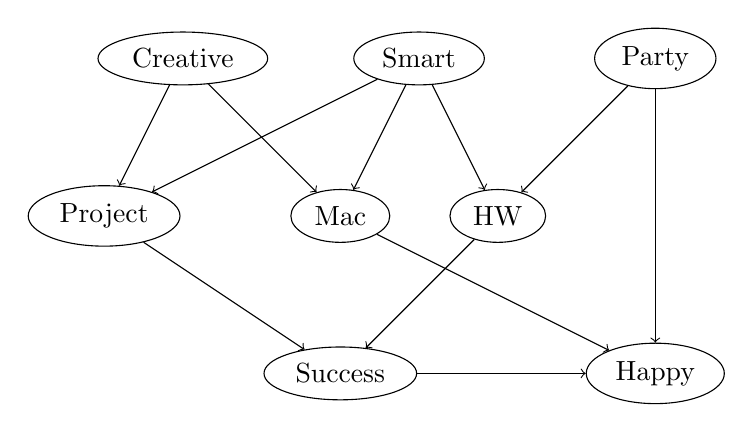
\begin{tikzpicture}
\usetikzlibrary{shapes}
\begin{scope}[every node/.style={ellipse,draw}]
\node (Creative) at (-3,2) {Creative};
\node (Project) at (-4,0) {Project};
\node (Mac) at (-1,0) {Mac};
\node (HW) at (1,0) {HW};
\node (Smart) at (-0,2) {Smart};
\node (Success) at (-1,-2) {Success};
\node (Happy) at (3,-2) {Happy};
\node (Party) at (3,2) {Party};
\end{scope}

\begin{scope}[every edge/.style={draw}]
    \path [->] (Creative) edge (Project);
    \path [->] (Creative) edge (Mac);
    \path [->] (Smart) edge (Project);
    \path [->] (Smart) edge (Mac);
    \path [->] (Smart) edge (HW);
    \path [->] (Party) edge (HW);
    \path [->] (Party) edge (Happy);
    \path [->] (Project) edge (Success);
    \path [->] (Mac) edge (Happy);
    \path [->] (HW) edge (Success);
    \path [->] (Success) edge (Happy);
\end{scope}
\end{tikzpicture}
\end{center}
\end{figure}


\begin{itemize}
\item \textbf{Q:} True or False: $Party$ is independent of $Success$ given $HW$. 

\begin{solution}
\textbf{A:}  False; there is a path that is not blocked:  
 $Party - HW - Smart - Project - Success$ has neither a converging arrows
not in the set of evidence or a non-converging arrows in
the set.\\
\end{solution}

\ifthenelse{\boolean{solutionCopy}}{}{\vspace{2cm}}

\item \textbf{Q:} True or False: $Creative$ is independent of $Happy$ given $Mac$. 

\begin{solution}
\textbf{A:}  False; there is a path that is not blocked: 
 $Creative -  Project - Success - Happy$\\
\end{solution}

\ifthenelse{\boolean{solutionCopy}}{}{\vspace{2cm}}

\item \textbf{Q:} True or False: $Party$ is independent of $Smart$  given $Success$. 

\begin{solution}
\textbf{A:} False; there is a path that is not blocked between $Party$ and $Smart$:
the path $Party - HW - Success$ is not blocked because the converging arrows
node at $HW$ has a descendant ($Success$) in the evidence.\\
% through the converging arrows at $HW$, which is activated by $Success$.\\
\end{solution}

\ifthenelse{\boolean{solutionCopy}}{}{\vspace{2cm}}

\item \textbf{Q:} True or False: $Party$ is independent of $Creative$  given $Happy$. 

\begin{solution}
\textbf{A:} False; there is a path that is not blocked between $Party$ and $Creative$ through the converging arrows at $Happy$. There are actually multiple not-blocked paths -- can you find them?\\
\end{solution}

\ifthenelse{\boolean{solutionCopy}}{}{\vspace{2cm}}

\item \textbf{Q:} True or False: $Party$ is independent of $Creative$  given $Success$, $Project$
and $Smart$.

\begin{solution}
\textbf{A:} True! All paths between  $Party$ and $Creative$ are blocked. 
Working from $Party$, the paths that come through $Happy$
are blocked there (converging arrows, no evidence). Those that come through $HW$ and $Smart$ are blocked 
at $Smart$. Those that come through $HW, Success, Project$ are blocked at $Project$.
\end{solution}

\ifthenelse{\boolean{solutionCopy}}{}{\vspace{2cm}}

\end{itemize}

\newpage
\section{Inference}
Consider the following Bayesian network, where all variables are Bernoulli.

\begin{figure}[htp]
% \begin{center}
%  \includegraphics[width=6in]{picture3.png}\\
%  \end{center}
 \begin{center}
$$\vspace{-1in}$$
 \begin{tikzpicture}
\begin{scope}[every node/.style={circle,draw}]
\node[label={180:\small $p(A=true)=0.2$}] (A) at (-2,1) {$A$};
\node[label={[label distance=-1cm]90:\small $p(B=true)=0.5$}] (B) at (0,1) {$B$};
\node[label={0:\small $p(C=true)=0.8$}] (C) at (2,1) {$C$};
\node (D) at (-1,-1) {$D$};
\node (E) at (1,-1) {$E$};
\end{scope}

\begin{scope}[every edge/.style={draw}]
    \path [->] (A) edge (D);
    \path [->] (B) edge (D);
    \path [->] (B) edge (E);
    \path [->] (C) edge (E);
\end{scope}
\end{tikzpicture}

\vspace{0.5cm}

\begin{tabular}{cc|c}
$A$ & $B$ & $p(D=true | A,B)$ \\
\hline
$F$ & $F$ & 0.9 \\
$F$ & $T$ & 0.6 \\
$T$ & $F$ & 0.5 \\
$T$ & $T$ & 0.1 \\
\end{tabular}
\quad
\begin{tabular}{cc|c}
$B$ & $C$ & $p(E=true | B,C)$ \\
\hline
$F$ & $F$ & 0.2 \\
$F$ & $T$ & 0.4 \\
$T$ & $F$ & 0.8 \\
$T$ & $T$ & 0.3 \\
\end{tabular}
\end{center}
\end{figure}

\begin{itemize}
\item \textbf{Q:} What is the probability that all five variables are simultaneously $false$? 

\begin{solution}
\textbf{A:}  
%
\begin{align*}
p(\neg A, \neg B, \neg C, \neg D, \neg E) &= p(\neg A) p(\neg B) p(\neg C) p(\neg D|\neg A, \neg B) p(\neg E | \neg B, \neg C)\\
&= (0.8)(0.5)(0.2)(0.1)(0.8)\\
&= 0.0064
\end{align*}
\end{solution}

\ifthenelse{\boolean{solutionCopy}}{}{\vspace{4cm}}

\item \textbf{Q:} What is the probability that $A$ is $false$ given that the remaining variables are all known to be $true$? \\

\begin{solution}
\textbf{A:} For this part, we need to calculate $p(\neg A|B,C,D,E)$. 

%We know that $p(\neg A|B,C,D,E) \propto p(\neg A,B,C,D,E)$. The joint probabilities $p(\neg A,B,C,D,E)$ and  $p(A,B,C,D,E)$ can be computed as:
By the definition of conditional probability, $$p(\neg A|B,C,D,E) = \frac{p(\neg A,B,C,D,E)}{P(B,C,D,E)} = \frac{p(\neg A,B,C,D,E)}{P(\neg A, B,C,D,E) +P(A, B,C,D,E)  } $$ The joint probabilities $p(\neg A,B,C,D,E)$ and  $p(A,B,C,D,E)$ can be computed as:
%
%Because $p(A,B,C,D,E) = p(A)p(B)p(C)p(D|A,B)p(E|B,C)$, we have:
\begin{align*}
p(\neg A,B,C,D,E) &= p(\neg A)p(B)p(C)p(D|\neg A,B)p(E|B,C)\\
&=(0.8)(0.5)(0.8)(0.6)(0.3) \\
&=(0.05760) \\
p(A,B,C,D,E)&= p(A)p(B)p(C)p(D| A,B)p(E|B,C)\\
&=(0.2)(0.5)(0.8)(0.1)(0.3)\\
&=(0.00240) 
\end{align*}

Finally, we can plug this in to get:
%
\begin{align*}
p(\neg A| B,C,D,E) = \frac{.05760}{.05760 +.00240} = .96
\end{align*}
\end{solution}

\end{itemize}

\section{Brainstorm Practical 3 (10min)}
\end{document}

%%% Local Variables:
%%% mode: latex
%%% TeX-master: t
%%% End:
